%=============================================================================
\chapter{MNRU: Modulated Noise Reference Unit}
%=============================================================================

For evaluation of the quality of a system or equipment, it is important to express the quality measure in a unit
suitable for comparison with other reference (or well-known) equipments and systems.
A common way of representing these figures is by means of relative units, where the quality is expressed by means of a
unique figure, in a unidimensional scale.

But it is insufficient to be unidimensional; the scale must be inequivocal, with a universal meaning.
As an example, the ACR scale ({\em Absolute Category Rating}, \cite[Annex B]{P.800}), which is a scale used for
listening opinion tests and has five points termed {\em Excellent}, {\em Good}, {\em Fair}, {\em Poor}, and {\em Bad},
is inadequate: besides it shows a continuum of quality points, the meaning of the adjectives are far from universal,
varying from language to language, and from person to person.
Exchange of information on the performance of these systems and equipments is easier and more consistent with more
objective measures.
The issue of how the MNRU is to be used as a reference system in subjective tests has been studied in ITU-T Study Group
12, which is described in Recommendation ITU-T P.830 \cite{P.830} in its Sections 8.2.2 and 11.

The Modulated Noise Reference Unity (MNRU) was introduced as a means to control degradations that are representative
of the non-linear distortion introduced by waveform coding techniques.
Initially aiming at evaluating the quality of log-PCM waveform coding systems, it has been used in the process of
generating several ITU-T standards, such as the ITU-T G.726 (32 kbit/s), G.722, G.728, and G.729.

The concept of such reference unit was published in \cite{Q001.02.04.02}.
The first system aimed at was the PCM coding with logarithmic compression (today world-wide available by means of the
Recommendation ITU-T G.711), whose main characteristic is to have a considerably uniform signal-to-noise ratio (SNR)
over a wide range of amplitudes.
Moreover, the quantizing noise is correlated to the signal: if no signal is present, no quantization noise is
produced\footnote{\SF This is obviously academic, because always there will be idle noise, among others, in the absence
of an input signal.}, and large signals will produce more quantization noise than small ones.
Therefore, the main characteristic of this reference unit should output speech corrupted by a speech-correlated noise.

%------------------------------------------------------------------------
% P.810 narrow-band MNRU
% The box y-length has been decreased by 1cm and the ps data
%  shifted down by ~1cm (-18 points)
%------------------------------------------------------------------------
 \begin{figure}[hpbt]
  \begin{center}
    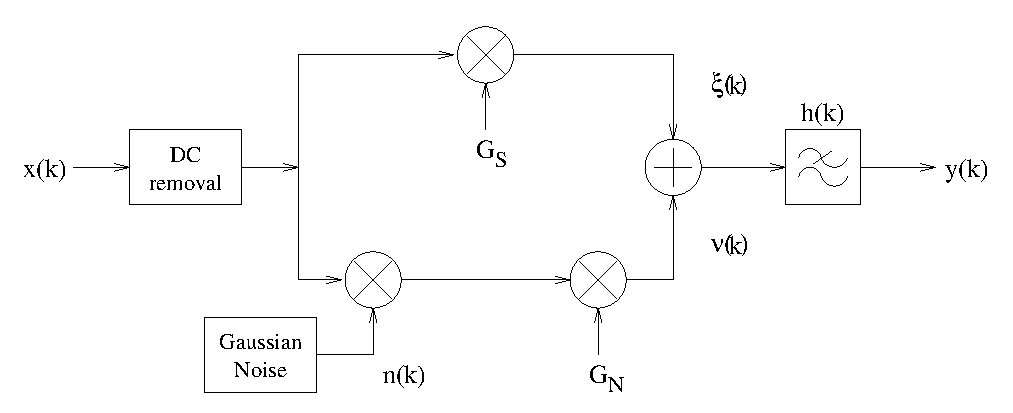
\includegraphics{p81-dig}
  \end{center}
  \caption{Block diagram of the ``digital'' MNRU. The bandwidth of the output filter $h(k)$ is 0--3400 Hz for the
  narrowband case, and 0--7000 Hz for the wideband case. \label{1/P.810}}
 \end{figure}
%------------------------------------------------------------------------

In \cite{Q001.02.04.02}, the speech-correlated noise generation was based on a double-balanced ring modulator,
controlled by the input speech signal, which modulates a noise carrier generated by a noise generator having a
relatively uniform energy distribution, there in the range of 0--20kHz.
This correlated noise is then added to the input signal, with gains applied such that a controlled signal-to-noise
ratio is obtained in the output, after the 300--3400Hz band-limiting filter.

With the 1996 revision of the MNRU description published in Recommendation ITU-T P.810\footnote{\SF Formerly known as
Recommendation ITU-T P.81.}, specific
guidelines were given for ``digital implementations''\footnote{\SF The revised
P.81 define a ``digital implementation'' either as a digital hardware implementation or as a software implementation of
the MNRU.}, eliminating many of the ambiguities
possible in earlier descriptions \cite{Old-P.81}, as explained in the STL92 manual
\cite[Chapter 8]{STL92-Manual}. Figure \ref{1/P.810} shows a block diagram of the ``digital'' MNRU.
Also, this implementation allows for transparent operation on narrowband or wideband speech, hence being known as
Dual-mode MNRU, or ``Duo-MNRU'', for short.

In 2008, Swissqual introduced a full-band MNRU algorithm, known as P.50 MNRU, to provide controlled super-wideband and
full-band MNRU degradations.
The algorithm adds a filtering stage that shapes the white noise according to an average speech power spectrum as
in \cite{P.50} to reduce the impact of the noise in the high-frequencies.
This algorithm was used in several standardization efforts, notably for the standardization of ITU-T Rec. P.863 \cite{P.863}
and EVS \cite{EVS}.
ITU-T Rec. P.810 was updated in 2022 with an implementation of the P.50 full-band MNRU described in \ref{fullband}.

\section{Dual-mode Modulated Noise Reference Unit - Narrowband and wideband speech}

\subsection{Description of the Algorithm}

The de-facto reference implementation of the MNRU\footnote{\SF Developed by the British Telecom and licenced to Malden
Electronics.} is the same of the original description, whose
specification can be found in Recommendation ITU-T P.810 \cite{P.810} (formerly Recommendation ITU-T P.81 \cite{Old-P.81}).
This Recommendation describes two MNRU schemes, one called {\em Narrow-band MNRU}, and another, {\em Wideband MNRU}.
Wideband MNRU is applicable to systems where wideband speech (70--7000Hz) is expected, whereas Narrow-band MNRU is for
telephone bandwidth (300--3400Hz).
Both narrowband and wideband MNRUs are implemented in this version of the ITU-T Software Tools Library.

The basic block diagram of the P.810 MNRU is found in figure\ref{1/P.810}.
In summary, there are two paths, one called {\em signal path}, another called {\em noise path}.
In the noise path, gaussian noise (uniform in a range at least the cutoff frequency of the low-pass filter in the
output of the MNRU) is modulated by the incoming signal.
The result is then added with the output from the signal path.
The gains are set such that the gain (in dB) applied in the output of the noise path is the signal-to-correlated-noise
ratio $Q$, in the output of the band-pass filter, as calculated in the section to follow.

In analytical terms, the signal corrupted by the modulated noise $y(k)$ is
\[
       y(k) = (G_s x(k) + G_n x(k) n(k)) \ast h(k)
\]
where $G_s$ is the gain of the signal path, $G_n$ is the gain of the noise path, $x(k)$ is the input signal, and $n(k)$
is the gaussian noise signal; the symbol $\ast$ means convolution, and $h(k)$ is the band-pass filter.

If we suppose that the band-pass filter has $|H(f)|=1$ in its pass band, and calling $Q$ the signal-to-noise-ratio (SNR)
at its output, we may write:
\[
    10^{Q/10} = \frac{\sigma^2_\xi}{\sigma^2_\nu} =
                \frac{E[\xi^2(k)]}{E[\nu^2(k)]}=
                \frac{G^2_s E[x^2(k)]}{G^2_n E[x^2(k) n^2(k)]}
\]
But $x$ and $n$ are uncorrelated, and the noise is gaussian with mean 0 and variance 1 (N(0,1)):
\[
    10^{Q/10} = \left( \frac{G_s}{G_n} \right)^2
                \frac{\sigma^2_x}{\sigma^2_x \sigma^2_n} =
                \left( \frac{G_s}{G_n} \right)^2
\]
or
\[
\begin{array}{lll}
     Q &= &\Gamma_s + \Gamma_n \\
     \Gamma_s &= &20 \log_{10}(G_s)\\
     \Gamma_n &= &-20 \log_{10}(G_n)
\end{array}
\]

If we set $\Gamma_s=0$ ($G_s=1$), $Q$ is exactly $\Gamma_n$ (or, $G_n=10^{-Q/20}$), i.e., the SNR is the gain (in dB) of the noise
path and the previous expression may be written as:
\[
y(k)=[x(n)+10^{-Q/20} x(k) n(k)] \ast h(k)
\]
or approximately
\[
y(k)=x(k)+10^{-Q/20} x(k) n(k)
\]
in the passband region of $H(f)|$.

When both $G_s$ and $G_n$ are non-zero, the MNRU is in an operational mode normally called {\em Modulated-noise mode}.
This is the most common operation mode.

Alternatively, if one consider $G_s=0$, the output of the algorithm is only the correlated noise, at a level $Q$ dB below the input signal.
This is {\em Noise-only mode}.

If, on the other hand, $G_n=0$, the output of the algorithm is the input signal filtered by $h(k)$, with a gain $G_s$;
this is the {\em Signal-only mode}.

\subsection{Implementation}

This implementation of the MNRU algorithm can be found in the module {\tt mnru.c}, with prototypes in {\tt mnru.h}.
A thorough characterization of this module is presented in \cite{Duo-MNRU}.

%------------------------------------------------------------------------
% Rev.P.81 MNRU, as implemented in the STL96
% The original .fig file has NOT been scaled
%  and the box y-length has been decreased by 1cm and the ps data
%  shifted down by ~1cm (-18 points)
%------------------------------------------------------------------------
\begin{figure}[ht]
  \begin{center}
    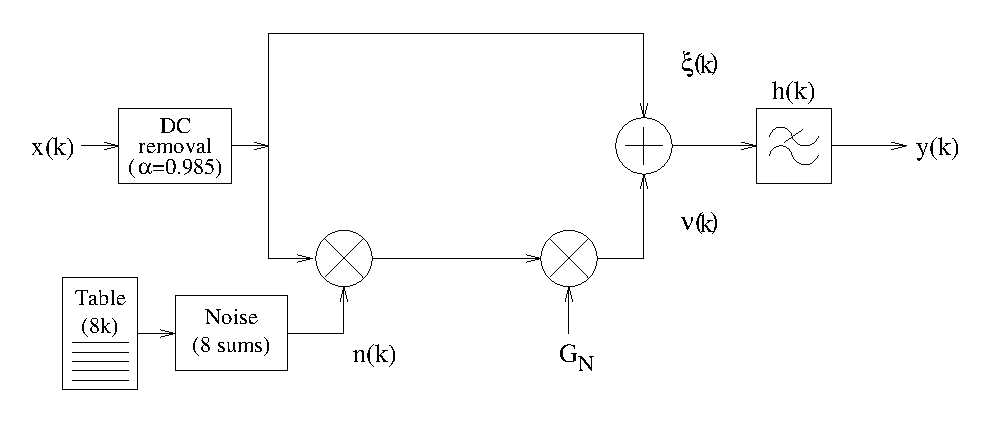
\includegraphics{p81-impl}
  \end{center}
   \caption{STL MNRU implementation.\label{STL96-MNRU}}
\end{figure}
%------------------ End of test of figure ----------------------------------

The block diagram of the MNRU implemented in the STL is in figure \ref{STL96-MNRU}.

The MNRU works internally on a sample-by-sample basis but for ease of interface with other speech coding functions,
access to it is made on a sample block basis.
It should be noted however that the filters have memory, as well as do the random number generator, hence state
variables are needed.
These state variables have been arranged as fields of a structure whose {\tt type} name is {\tt MNRU\_state}.
The fields of the structure are:
\begin{quote} \normalsize
 {\em seed}     \hfill \parbox{100mm}{\SF RNG's seed }\\
 {\em signal\_gain}     \hfill \parbox{100mm}{\SF Gain of the signal path }\\
 {\em noise\_gain}      \hfill \parbox{100mm}{\SF Gain of the noise path }\\
 {\em vet}      \hfill \parbox{100mm}{\SF Array for intermediate data }\\
 {\em last\_xk} \hfill \parbox[t]{100mm}{\SF $x(k-1)$ used as memory for
                            the DC-removal filter }\\
 {\em last\_yk}\hfill \parbox[t]{100mm}{\SF $\xi(k-1)$ (see figure
                            \ref{STL96-MNRU}), used as memory for the
                            DC-removal filter}\\
 {\em DLY[2][2]}      \hfill \parbox[t]{100mm}{\SF Memory of delayed
                            samples for two second-order stages (first
                            index) for first- and second-order delays
                            (second index)}\\
 {\em A[2][2]}  \hfill \parbox[t]{100mm}{\SF Numerator coefficients for
                            the stage indicated by the first index and
                            delay-order inidcated by the second index}\\
 {\em B[2][2]}  \hfill \parbox[t]{100mm}{\SF Denominator coefficients for
                            the stage indicated by the first index and
                            delay-order inidcated by the second index}\\
 {\em rnd\_state}  \hfill \parbox[t]{100mm}{\SF State structure for MNRU's
                            random number generator. Detailed
                            description is found in the section on the
                            random number generator.}\\
 {\em rnd\_mode}   \hfill \parbox[t]{100mm}{\SF Operational mode of the
                            random number generator}\\
 {\em clip}     \hfill \parbox[t]{100mm}{\SF Number of samples clipped in
                            the noise-insertion process}\\
\end{quote}

The values of the fields shall not be altered by the user.


%----------------------------------------------------------------------------
\subsubsection{Filters in the MNRU module}

The composite frequency response of the narrowband and wideband MNRU filters is shown in figure \ref{MNRU:both-filters}.
Figure \ref{MNRU:lp-filter} shows the contribution of the output low-pass filter for (a) the narrowband, and (b) the
wideband cases.
Figure \ref{MNRU:hp-filter} shows the effect of the input DC-removal filter for (a) the narrowband and (b) the wideband
operation modes of the MNRU.
Details on the design of the output low-pass filters are given in \cite{Duo-MNRU}.
The frequency responses have been obtained by exciting the MNRU module with digital sinewaves and computing the ratio
of input and output signals, in dB.


%---------------------------------------------------------------------
% Frequency response of MNRU filters: Both filters convolved
%---------------------------------------------------------------------
%mnrufrnb.ps: narrowband, full-filter
%Box dimension: 12.06cm x 10.48cm
%mnrufrwb.ps: wideband, full-filter
%Box dimension: 12.06cm x 10.48cm
%---------------------------------------------------------------------
\begin{figure}[p]
  \begin{center}
    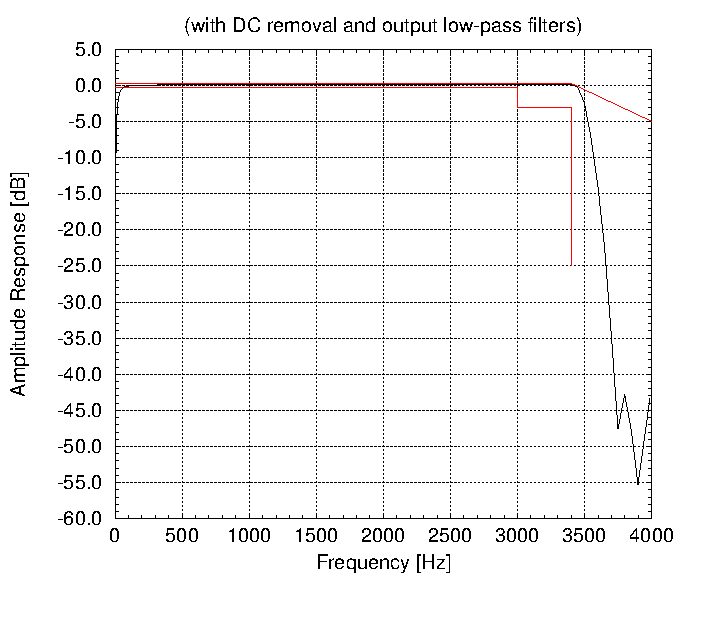
\includegraphics{mnrufrnb}
    \\
    (a) Narrowband Duo-MNRU

    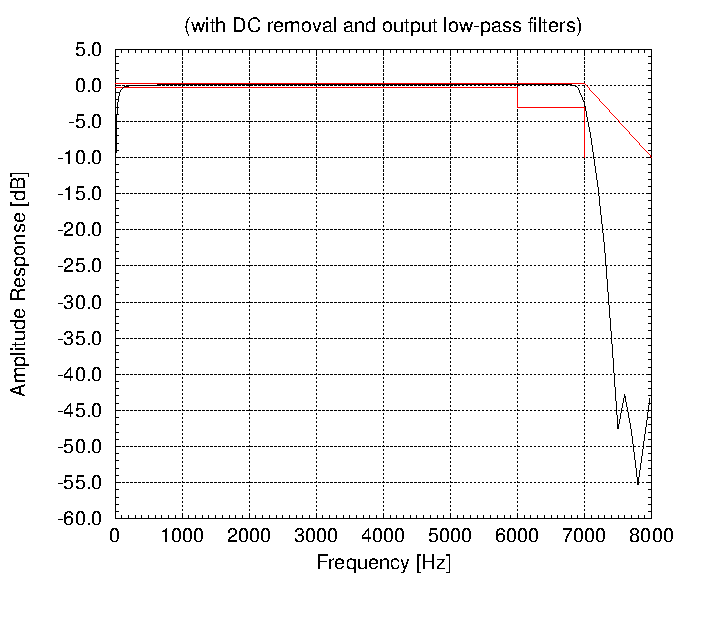
\includegraphics{mnrufrwb}
    \\
    (b) Wideband Duo-MNRU
  \end{center}
  \caption{ Total frequency response of the Duo-MNRU filters.
            \label{MNRU:both-filters}
          }
\end{figure}
%----------------------------------------------------------------------

%----------------------------------------------------------------------
% Frequency response of MNRU filters: zoom of LP part
%----------------------------------------------------------------------
%mnrudcnb.ps: narrowband, DC-removal HP filter
%Box dimension: 12.06cm x 10.48cm
%mnrudcwb.ps: wideband, DC-removal HP filter
%Box dimension: 12.06cm x 10.48cm
%----------------------------------------------------------------------
\begin{figure}[p]
  \begin{center}
    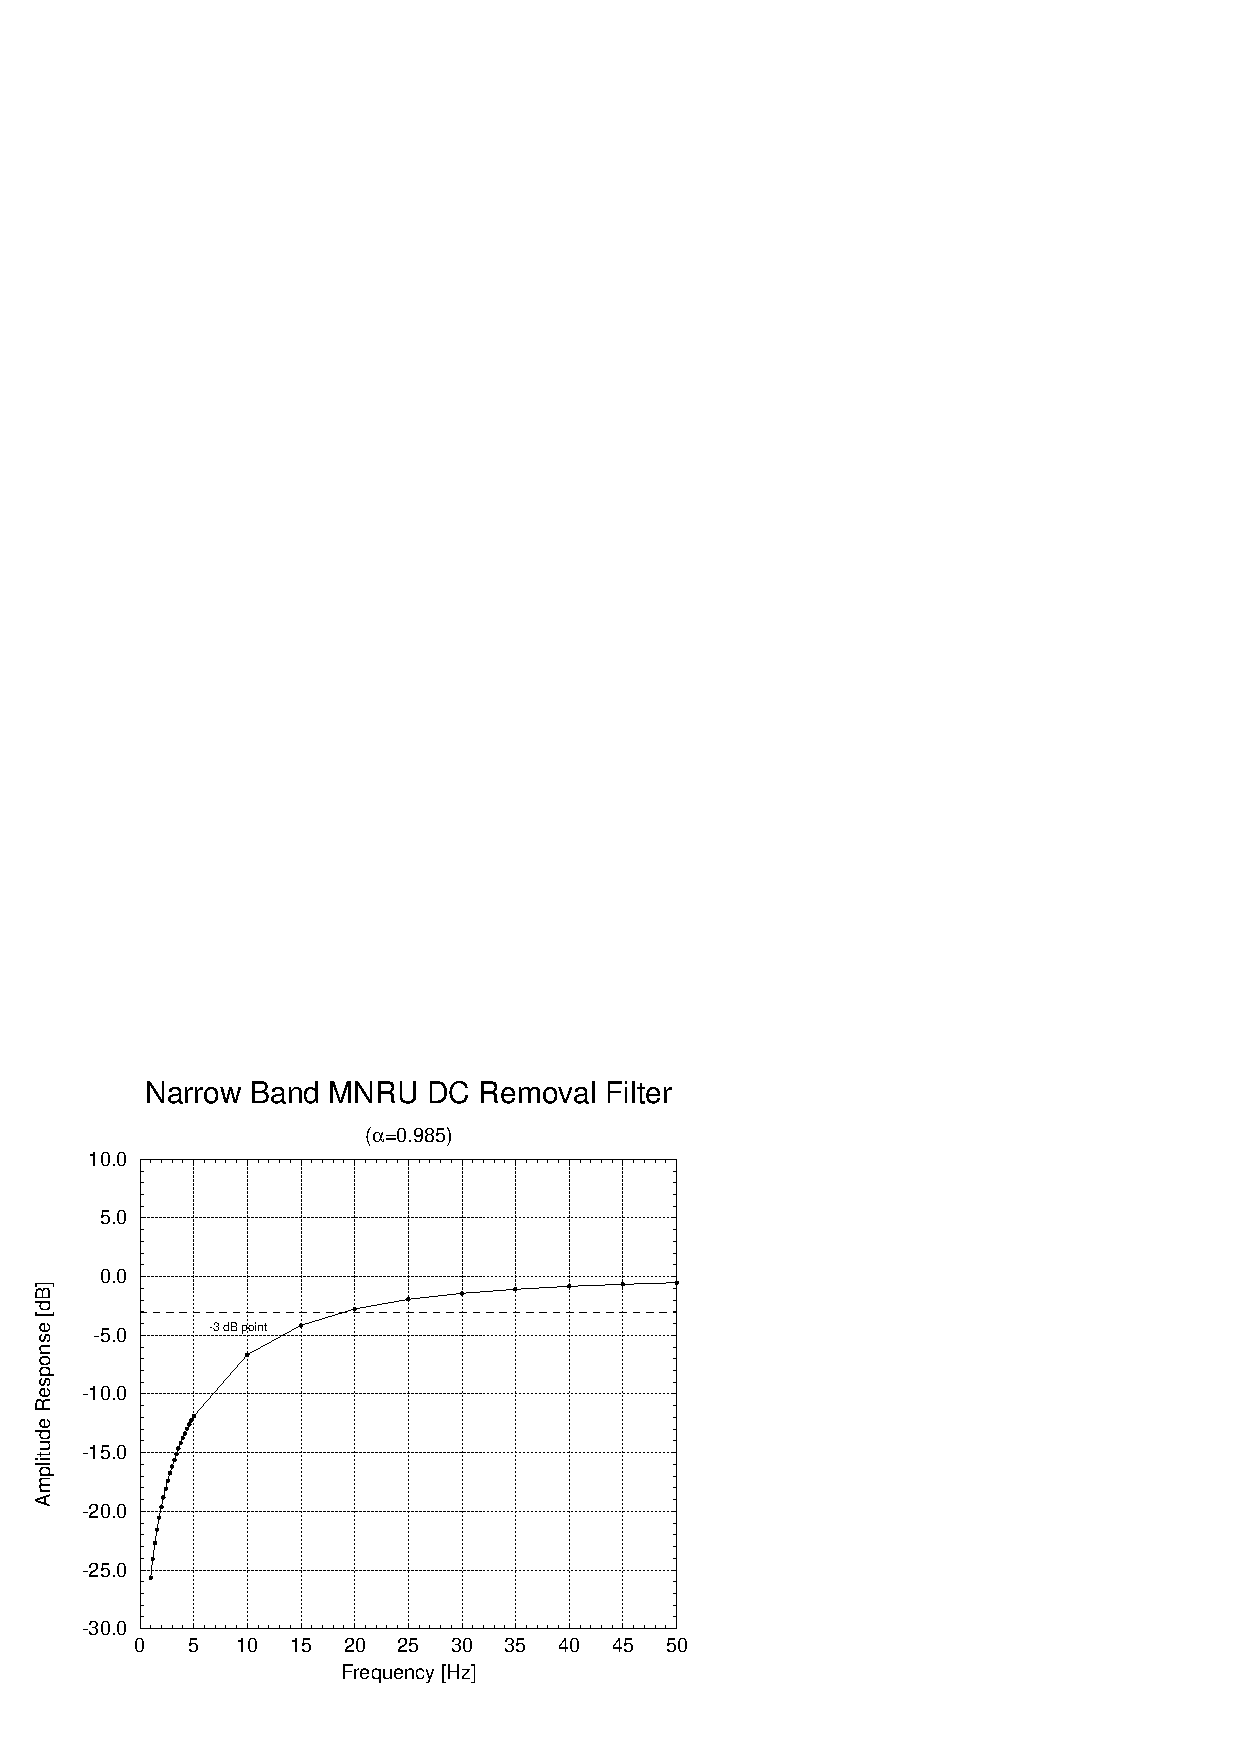
\includegraphics{mnrudcnb}
    \\
    (a) Narrowband Duo-MNRU

    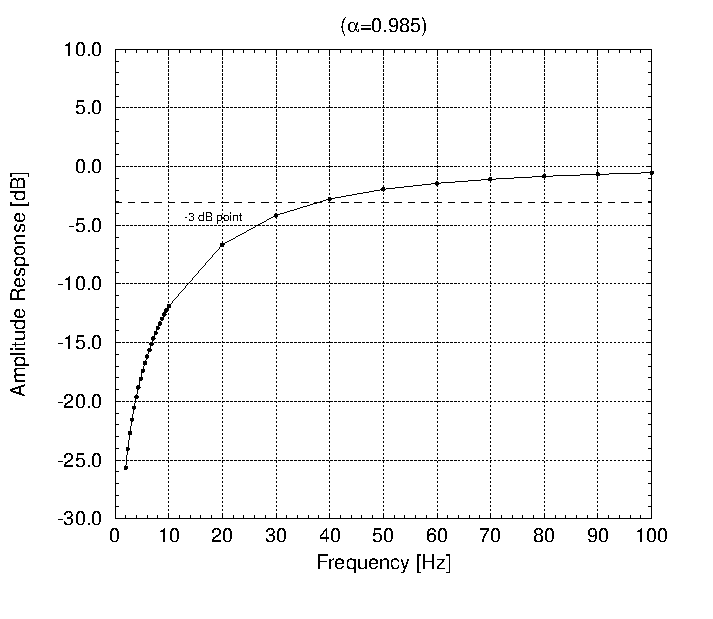
\includegraphics{mnrudcwb}
    \\
    (b) Wideband Duo-MNRU
  \end{center}
  \caption{ DC removal filter for the Duo-MNRU. \label{MNRU:hp-filter} }
\end{figure}
%-----------------------------------------------------------------------

%-----------------------------------------------------------------------
% Frequency response of MNRU filters: zoom of DC (HP) part
%-----------------------------------------------------------------------
%mnrulpnb.ps: narrowband, output LP filter
%Box dimension: 12.06cm x 10.48cm
%mnrulpwb.ps: wideband, output LP filter
%Box dimension: 12.06cm x 10.48cm
%-----------------------------------------------------------------------
\begin{figure}[hp]
  \begin{center}
    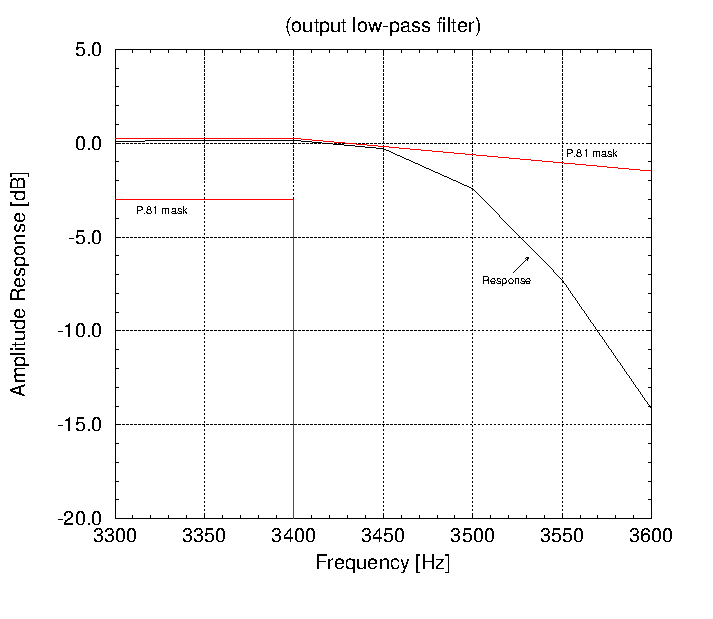
\includegraphics{mnrulpnb}
    \\
    (a) Narrowband Duo-MNRU

    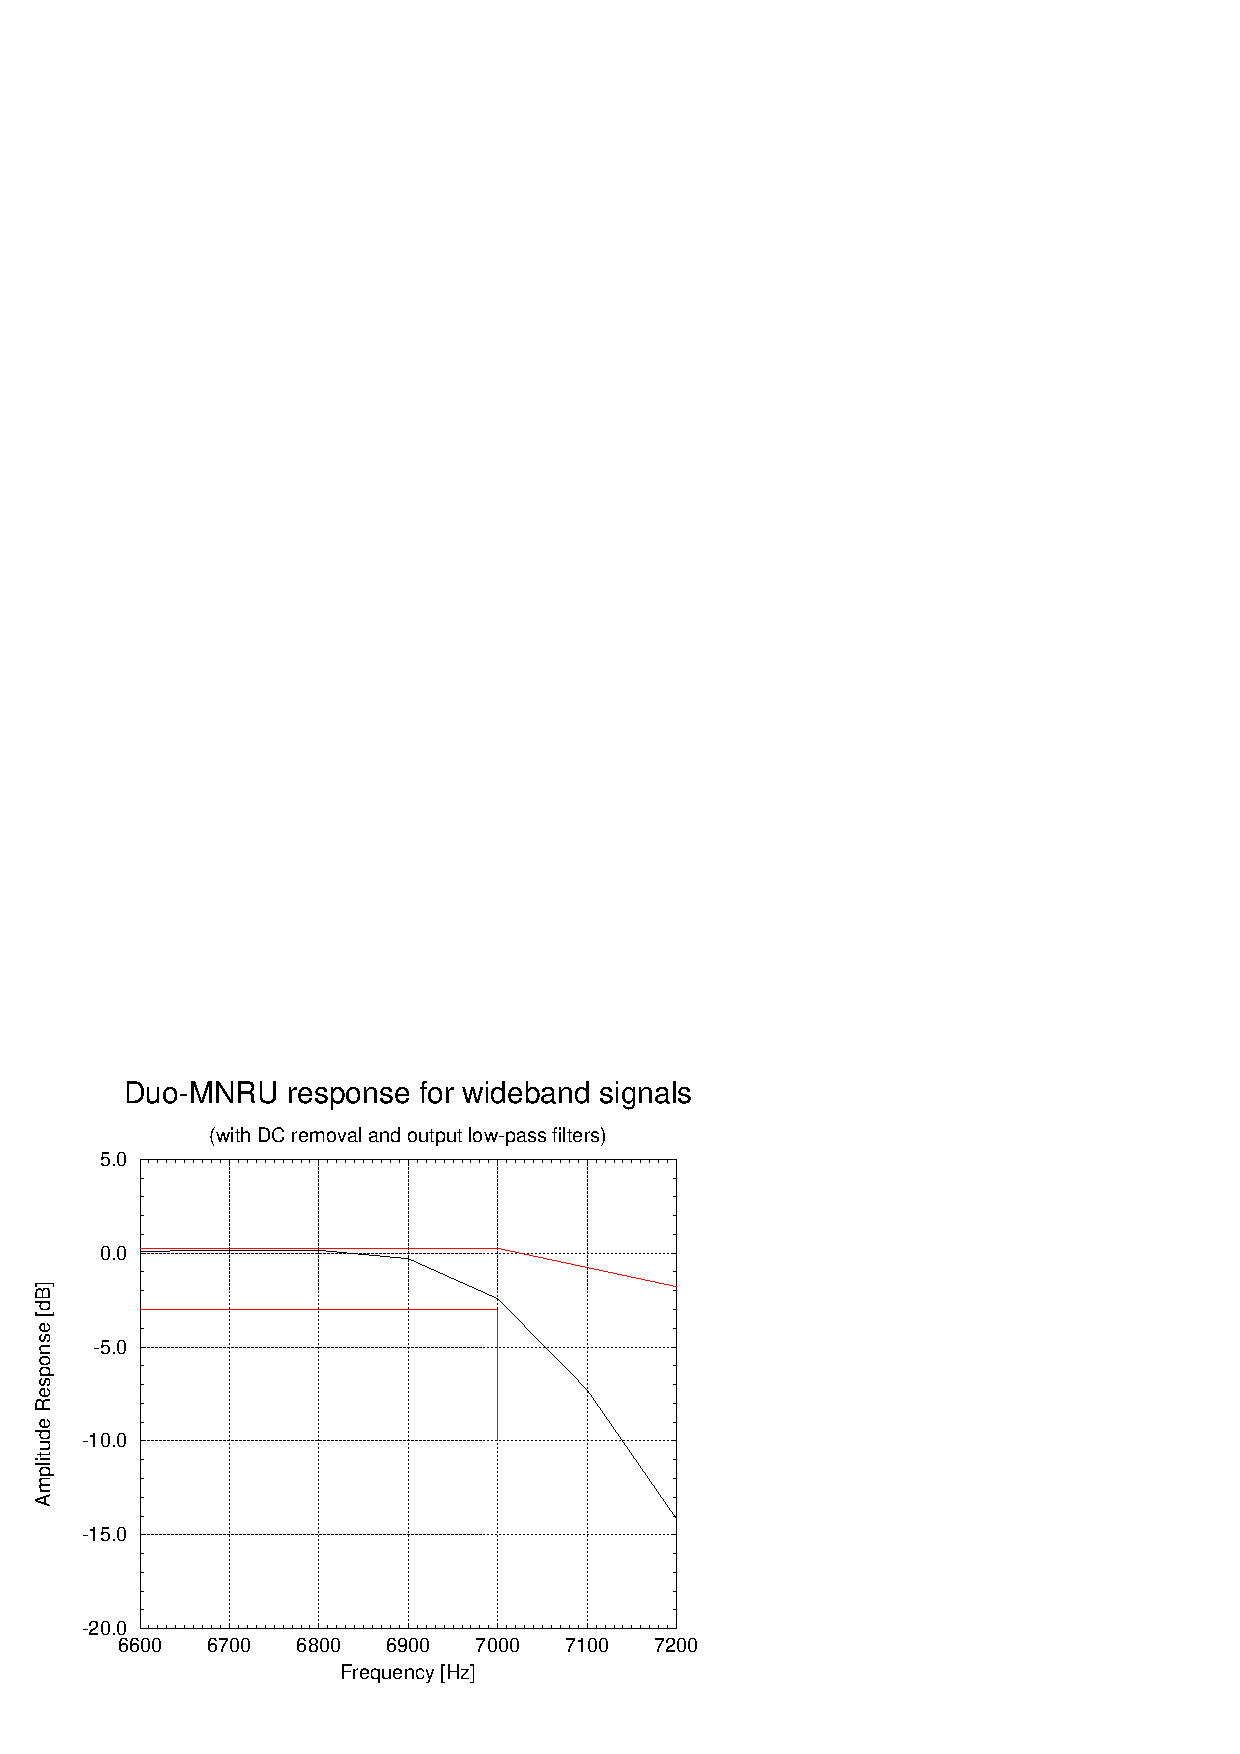
\includegraphics{mnrulpwb}
    \\
    (b) Wideband Duo-MNRU
  \end{center}
  \caption{ Output low-pass filter for the Duo-MNRU. \label{MNRU:lp-filter} }
\end{figure}
%-----------------------------------------------------------------------


%---------------------------------------------------------------------
% Filter structure of the MNRU
% The original box y-length has been decreased by 1cm and the ps data
%  shifted down by ~0.5cm (-10 points)
%---------------------------------------------------------------------
\begin{figure}[htb]
  \begin{center}
    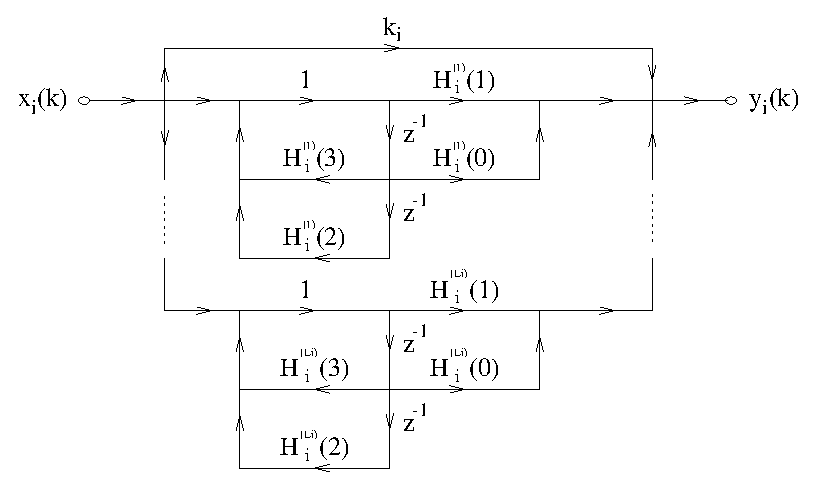
\includegraphics{mnru-iir}
  \end{center}
  \caption{MNRU Filters Structure.\label{MNRU-IIR}}
\end{figure}
%---------------------------------------------------------------------


The input DC-removal filter was implemented using a first-order IIR pole-zero filter defined by
\[
    H_i(z) = { 1-z^{-1} \over \ 1 - \alpha z^{-1} \ }
\]
with $\alpha$=0.985.
Its -3dB point is at 16 Hz for the narrowband case and at 38 Hz for the wideband case.

The output low-pass filter was implemented using a second-order cascade-form IIR filter with two-sections as illustrated
in figure \ref{MNRU-IIR} and defined by the equation:
\[
    H_i(z) = A \prod_{k=1}^{2}
                    { a_{0k}+a_{1k}z^{-1}+a_{2k}z^{-2} \over
                      \ 1+b_{1k}z^{-1}+b_{2k} z^{-2} \
                                }
\]

IIR filters were chosen because of their low computational complexity when compared to FIR implementations, allowing for
a more efficient MNRU implementation.


%------------------------------------------------------------------------------
\subsubsection{Random Number Generator for the MNRU module}

The random number generator (RNG) used in this implementation was chosen using the following criteria:

\rulex{5mm}
\begin{minipage}{130mm}
 $\bullet$ \parbox[t]{120mm}{
               the desired value for Q, $Q_d$, and the measured Q, $Q_m$, should be very close for a wide range of Q,
                e.g., Q from 0 to 50 dB.
               \bigskip}

 $\bullet$ \parbox[t]{120mm}{
               it should show a good approximation of a gaussian distribution.
               This is needed because it is specified in P.810 and more importantly because uniform distributions do not
               allow good matching between the desired and measured values of Q. \bigskip}

 $\bullet$ \parbox[t]{120mm}{
               the algorithm needed to be portable (i.e., identical results are got in different platforms if the same
                seed is given).}\\
\end{minipage}

The RNG chosen to be used in in STL92 version of the MNRU was based on Knuth's Subtractive Method \cite{Recipes},
\cite[Parts 3.2--3.3]{Knuth}, which generates adequate random sequences but is computationally intensive and was too
complex to be implemented in a real-time digital hardware MNRU.

The implementation used in the ITU-T G.729 8 kbit/s speech codec selection tests was based on a gaussian-noise table
lookup, in a manner similar to Malden Electronic's MNRU implementation.\footnote{\SF Malden's MNRU uses a ROM table
derived from  a Gaussian distribution with 4096 samples uniformly
distributed throughout the table. An address in the table is
uniformly sampled four times and accumulated to form a gaussian noise
sample.}
This approach is considerably less computationally intensive than the STL92 approach, and was used to further reduce the
complexity of the MNRU implementation.

After several experiments \cite{Duo-MNRU}, a table with 8192 gaussian samples was chosen to be used, which is randomly
and uniformly accessed 8 times (i.e., an eight-time sample accumulation) to be used by the MNRU algorithm.
The gaussian table itself is generated in run-time (rather than being stored in the data memory of the source or object
code) using the Monte-Carlo substitution algorithm.
The Monte-Carlo algorithm uses a linear congruential generation (LCG) algorithm defined by
\[
            I_{j} = 69069 I_{j-1} + 1 \pmod{2^{32}}
\]
which is converted to numbers in the range [0..1] using the upper 24 bits of the 32-bit unsigned long $I_j$.
$I_0$ is a fixed seed equal to 314159265.
This algorithm is used to generate the necessary initial random samples for the substitution algorithm.

Once the table has been filled, during the normal operation of the MNRU, eight successive samples are drawn (uniformily)
from the table using a different LCG algorithm
\[
            L_{j} = 253 L_{j-1} + 1 \pmod{2^{24}}
\]
of which the upper 13 bits are used to generate random numbers uniformly distributed between 0 and 8191. $L_0$ is a
fixed seed equal to 12345.
Both LCGs were implemented as in Aachen University's MNRU implementation.

Since different ranges are necessary for table filling and for gaussian sample generation, two different LCG random
number generators were used to avoid any additional calculations due to range convertion and to reduce the software load.

Since the Monte-Carlo RNG is used only at startup time, it is not necessary to keep any state variables for it.
The sample-drawing RNG however needs to keep stored the previously generated index, which is stored in a structure of
type {\tt RANDOM\_state}, whose only field is (as defined in {\tt mnru.h})\footnote{\SF The use of a structure
instead of a single variable in the parent structure ({\tt
MNRU\_state}) allows for unimplemented features to be easily added in
a later version of the algorithm.}:
\begin{quote} \normalsize
 {\em gauss}    \hfill \parbox{100mm}{\SF Index for next random number;}\\
\end{quote}

The field in {\tt RANDOM\_state} should not be altered by the user in any situation.

The operational modes are defined in {\tt mnru.h}:

\rulex{5mm} \parbox[t]{120mm}{\tt
\#define RANDOM\_RUN 0\\
\#define RANDOM\_RESET 1\\*[5mm]
}

The noise modulation routine is {\tt MNRU\_process}, which is described next.

\subsubsection{{\tt MNRU\_process}}

{\bf Syntax: }

{\tt
\#include "mnru.h"\\
double *MNRU\_process (\ttpbox{110mm}{
            char {\em operation}, {\tt MNRU\_state} {\em *s}, float {\em *input},
            float {\em *output}, long {\em n}, long {\em seed},
            char {\em mode}, double {\em Q});
         }
}

{\bf Prototype: }    mnru.h

{\bf Description: }

Module for addition of modulated noise to a vector of {\it n} samples, according to Recommendation ITU-T P.810, for
either the narrowband or the wideband model. Depending on the {\it mode}, this function:

\rulex{5mm}
\begin{minipage}{130mm}
 $\bullet$ \parbox[t]{120mm}{
           adds modulated noise to the {\it input} buffer at a SNR level of {\it Q} dB, saving to {\it output} buffer
          ({\it mode}=={\tt MOD\_NOISE});\\}

 $\bullet$ \parbox[t]{120mm}{
          puts into {\it output} only the noise, without addition of the original signal ({\it mode}=={\tt NOISE\_ONLY});\\}

 $\bullet$ \parbox[t]{120mm}{
          produces in the {\it output} a filtered-only (no noise added) version of the `input' samples ({\it mode}=={\tt SIGNAL\_ONLY});\\}

\end{minipage}

The symbols {\tt MOD\_NOISE}, {\tt NOISE\_ONLY}, and {\tt SIGNAL\_ONLY} are defined in {\tt mnru.h}.

Although the MNRU algorithm operates on a sample-by-sample basis, {\tt MNRU\_process} handles the input data in blocks
of {\it n} samples, for better computational efficiency.

The implementation of the MNRU algorithm has three operational states, called {\tt MNRU\_START}, {\tt MNRU\_CONTINUE} and
{\tt MNRU\_STOP}.
With {\tt MNRU\_START}, the state variables are set, as well as memory is allocated for the intermediate data, and this
needs to be the first operation with the algorithm.
Differently from the speech voltmeter module, after the initialization of the state variables, the normal calculations
are carried out for the first block of data.
Once reset, the algorithm changes the operation state to {\tt MNRU\_CONTINUE}, and the next calls to the MNRU algorithm
will skip the reset operation.
With the last block, it is adivisable to release the memory allocated to the intermediate data.
This is accomplished by calling {\tt MNRU\_process} with the operational state set as {\tt MNRU\_STOP}.
These three operational states are defined in {\tt mnru.h} as follows:

\rulex{5mm} \parbox[t]{120mm}{\tt
\#define MNRU\_START     1\\
\#define MNRU\_CONTINUE  0\\
\#define MNRU\_STOP     -1\\*[5mm]
}


{\bf Variables: }
\begin{Descr}{\DescrLen}
\item[\pbox{20mm}{\em operation}] %\rulex{1mm}\\
        One of the defined operation status:
        {\tt MNRU\_START}, {\tt MNRU\_STOP}, {\tt MNRU\_CONTINUE}.

\item[\pbox{20mm}{\em s}] %\rulex{1mm}\\
        A pointer to a {\tt MNRU\_state} structure.

\item[\pbox{20mm}{\em input}] %\rulex{1mm}\\
        Pointer to input float-data vector; must represent
                      8 or 16 kHz speech samples.

\item[\pbox{20mm}{\em output}] %\rulex{1mm}\\
        Pointer to output float-data vector; will represent
                      8 or 16 kHz speech samples.

\item[\pbox{20mm}{\em n}] %\rulex{1mm}\\
        Long with the number of samples (\float) in input.

\item[\pbox{20mm}{\em seed}] %\rulex{1mm}\\
        Initial value for random number generator.

\item[\pbox{20mm}{\em mode}] %\rulex{1mm}\\
        Operation mode: {\tt MOD\_NOISE}, {\tt SIGNAL\_ONLY}, {\tt NOISE\_ONLY} (description above).

\item[\pbox{20mm}{\em Q}] %\rulex{1mm}\\
        Double defining the desired value for the signal-to-modulated-noise $Q$ for the output data.
\end{Descr}

Please note that new values of {\em seed}, {\em mode}, and $Q$ are considered only when {\em operation} is {\tt MNRU\_START},
because they are considered as INITIAL state values.
Therefore, when the operation is not {\tt MNRU\_START}, they are ignored.


{\bf Return value: }

Returns a {\tt (double *)NULL} if not initialized or if initialization failed; returns a {\tt (double *)} to an
intermediate data vector if reset was successful or is in the {\tt MNRU\_CONTINUE} (``run'') operation state.


\subsection{Portability and compliance} \label{MNRU-Tests}

In the development of this module, several steps were taken to assure its compliance to Recommendation ITU-T P.810, which included:

\begin{itemize}
  \item agreement of expected and measured Q values for tones and speech,
  \item addition of partial files,
  \item level of output files,
  \item frequency response of built-in filters.
\end{itemize}

Additionally to these objective measurements, a subjective test was performed.
The results of this test are found in \cite{Duo-MNRU}, where it was concluded that the new MNRU implementation conforms
to the P.810 and also behaves more closely to the hardware MNRU than the previous STL92 version.

Additionally to the conformance tests, the algorithm was tested for portability using a 1kHz tone file as input to the
algorithm with Q values ranging from 0 to 50 dB in 5 dB steps, and also for the algorithm in the {\tt SIGNAL\_ONLY} mode.
The processed test files were then compared the the reference processed files (generated on a HP workstation). Test and
reference files should be identical.
The algorithm was found to compile and execute correctly on MS-DOS under Borland Turbo-C++ 1.0 and under the MS-DOS port
of the GNU-C compiler (gcc), on a HP UNIX workstation with cc (non-ANSI) and gcc, on a Sun workstation with cc (non-ANSI)
and also on VAX VMS and APX computers.


%-----------------------------------------------------------------
\subsection{Example code}

%.....................................................................
\subsubsection {Description of the demonstration programs}

One demonstration program is provided for the MNRU module, mnrudemo.c.
Irrespective of whether the 16-bit, linear PCM input file is sampled at 8 or 16 kHz, program {\tt mnrudemo.c} will add
the multiplicative noise signal to the input signal at the user-defined $Q$ level and produce as output a 16-bit, linear PCM file.
Optionally, the program can produce a signal-only file (equivalent to a very high Q value) or a noise-only file (the signal path is disconnected).

%These three modes of operation are provided for compatibility with the
%``classical'' hardware MNRU implementation.

%..........................................................................
\subsubsection {Simple example}

The following C code gives an example of a possible use of the Duo-MNRU module.
The input file speech is added to a multiplicative noise at a SNR defined by parameter Q.
All samples in the file are processed.

{\tt\small
\begin{verbatim}
#include <stdio.h>
#include <stdlib.h>
#include <math.h>
#include "ugstdemo.h"
#include "mnru.c"               /* ... Include MNRU module ... */
#include "ugst-utl.c"           /* ... Include of utilities ... */

#define BLK_LEN 256
main(argc, argv)
  int             argc;
  char           *argv[];
{
  /* File variables */
  char            FileIn[80], FileOut[80];
  FILE           *Fi, *Fo;
  MNRU_state      state;
  short           Buf[BLK_LEN];
  float           inp[BLK_LEN], out[BLK_LEN];
  double          QdB;
  long            l;
  char            MNRU_mode = MOD_NOISE, operation;

  /* Read parameters for processing */
  GET_PAR_S(1, "_Input File: ................. ", FileIn);
  GET_PAR_S(2, "_Output File: ................ ", FileOut);
  GET_PAR_D(3, "_Desired Q: .................. ", QdB);

  /* Check for parameter 4 to change MNRU operation mode */
  if (argc > 4)
  {
    MNRU_mode = toupper(argv[5][0]);
    if (MNRU_mode == 'S')       /* Signal-only mode */
      MNRU_mode = SIGNAL_ONLY;
    else if (MNRU_mode == 'M')  /* Modulated noise, the default mode */
      MNRU_mode = MOD_NOISE;
    else if (MNRU_mode == 'N')  /* Noise-only mode */
      MNRU_mode = NOISE_ONLY;
    else
    {
      fprintf(stderr, "Bad mode chosen; use M,N,or S \n"); exit(2);
    }
  }

  /* Opening input and output files */
  Fi = fopen(FileIn, RB);
  Fo = fopen(FileOut, WB);

  /* INSERTION OF MODULATED NOISE ACCORDING TO P.810 (FEB.96) */

  /* Set operation as start */
  operation = MNRU_START;

  /* Process for all samples in file */
  while ((l = fread(Buf, sizeof(short), BLK_LEN, Fi)) != NULL)
  {
    /* Convert data from 16-bit short to normalized float */
    sh2fl_16bit((long) l, Buf, inp, 1);

    /* MNRU processing */
    MNRU_process(operation, &state, inp, out, l, 314159265L, MNRU_mode, QdB);

    /* Change operation mode: START --> CONTINUE */
    if (operation == MNRU_START)
      operation = MNRU_CONTINUE;

    /* Convert from normalized float to short (hard clip and rounding) */
    fl2sh_16bit((long) l, out, Buf, 1);

    /* Save data to file */
    fwrite(Buf, sizeof(short), l, Fo);
  }

  /* Stop mode: Deallocation of memory, but process 0 samples */
  operation = MNRU_STOP;
  MNRU_process (operation, &state, inp, out, 0L, 0L, 0, (double) 0.0);

  /* Finalizations */
  fclose(Fi);
  fclose(Fo);
  return(0);
}

\end{verbatim}
}

\section{P.50 Fullband MNRU - Shaped noise spectrum for fullband speech signals} \label{fullband}

\subsection {Description}

In the case of fullband speech signals, the signal energy at higher frequencies is typically much weaker than in the
narrowband part of the spectrum.
Consequently, a modulated white noise signal will result in an uneven SNR across the signal spectrum.

In order to avoid higher amounts of perceived noise at high frequencies, the noise signal may be shaped in a pre-filtering
step such as to match the average spectrum of speech signals.
The filter frequency response can be derived from ITU-T Rec. P.50 \cite{P.50}, chapter 4 “Average voices – Long-term
average spectrum”, as shown in Figure \ref{MNRUP50}.

The overall structure of P.50 Fullband MNRU, shoing the additional filtering state of the noise source, is provided in
Figure \ref{MNRUP50FB}.

The diagram also shows that a control on the application of the DC removal filter.
It was observed that the DC filter in this implementation may alter the perception of the voice timber at high Q which
is undesirable.
Therefore it is recommended to use an external DC removal filter rather than using the implemented DC removal filter.
Since P.50 FB MNRU has been used with the DC removal filter enabled between 2008 and 2023, a switch is provided for
backward compatibility.

\begin{figure}[ht]
    \begin{center}
        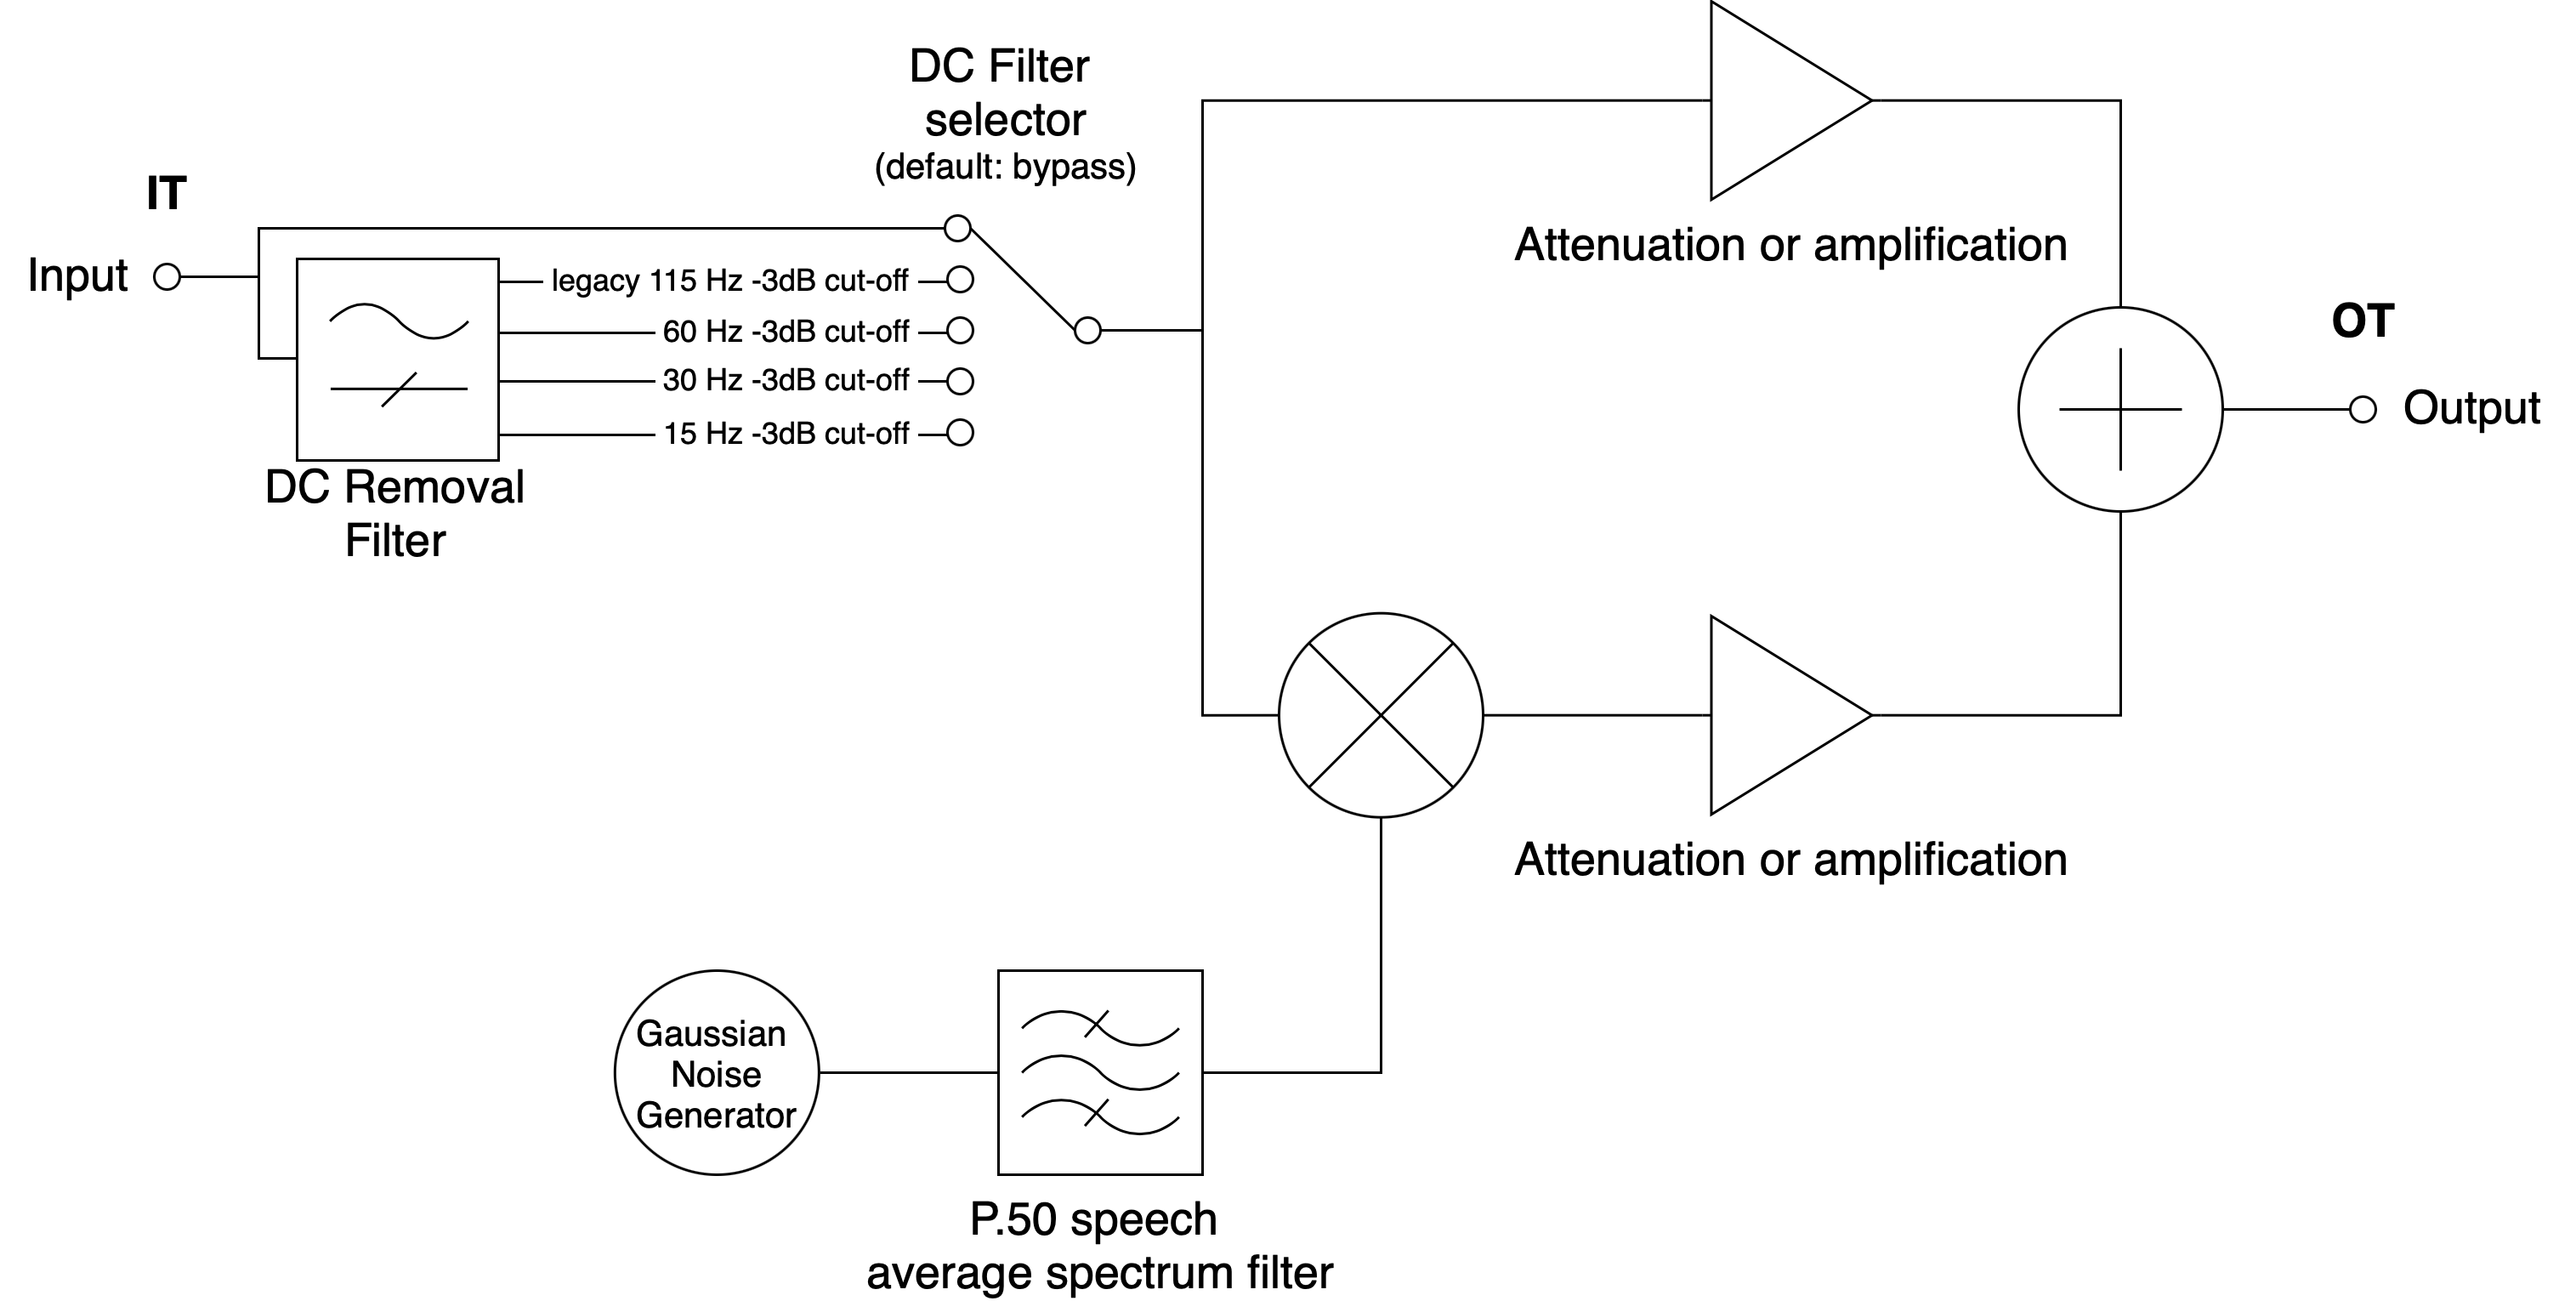
\includegraphics[width=\textwidth]{mnru-p50fb}
    \end{center}
    \caption{P.50 fullband MNRU implementation\label{MNRUP50FB}}
\end{figure}

\begin{figure}[ht]
    \begin{center}
        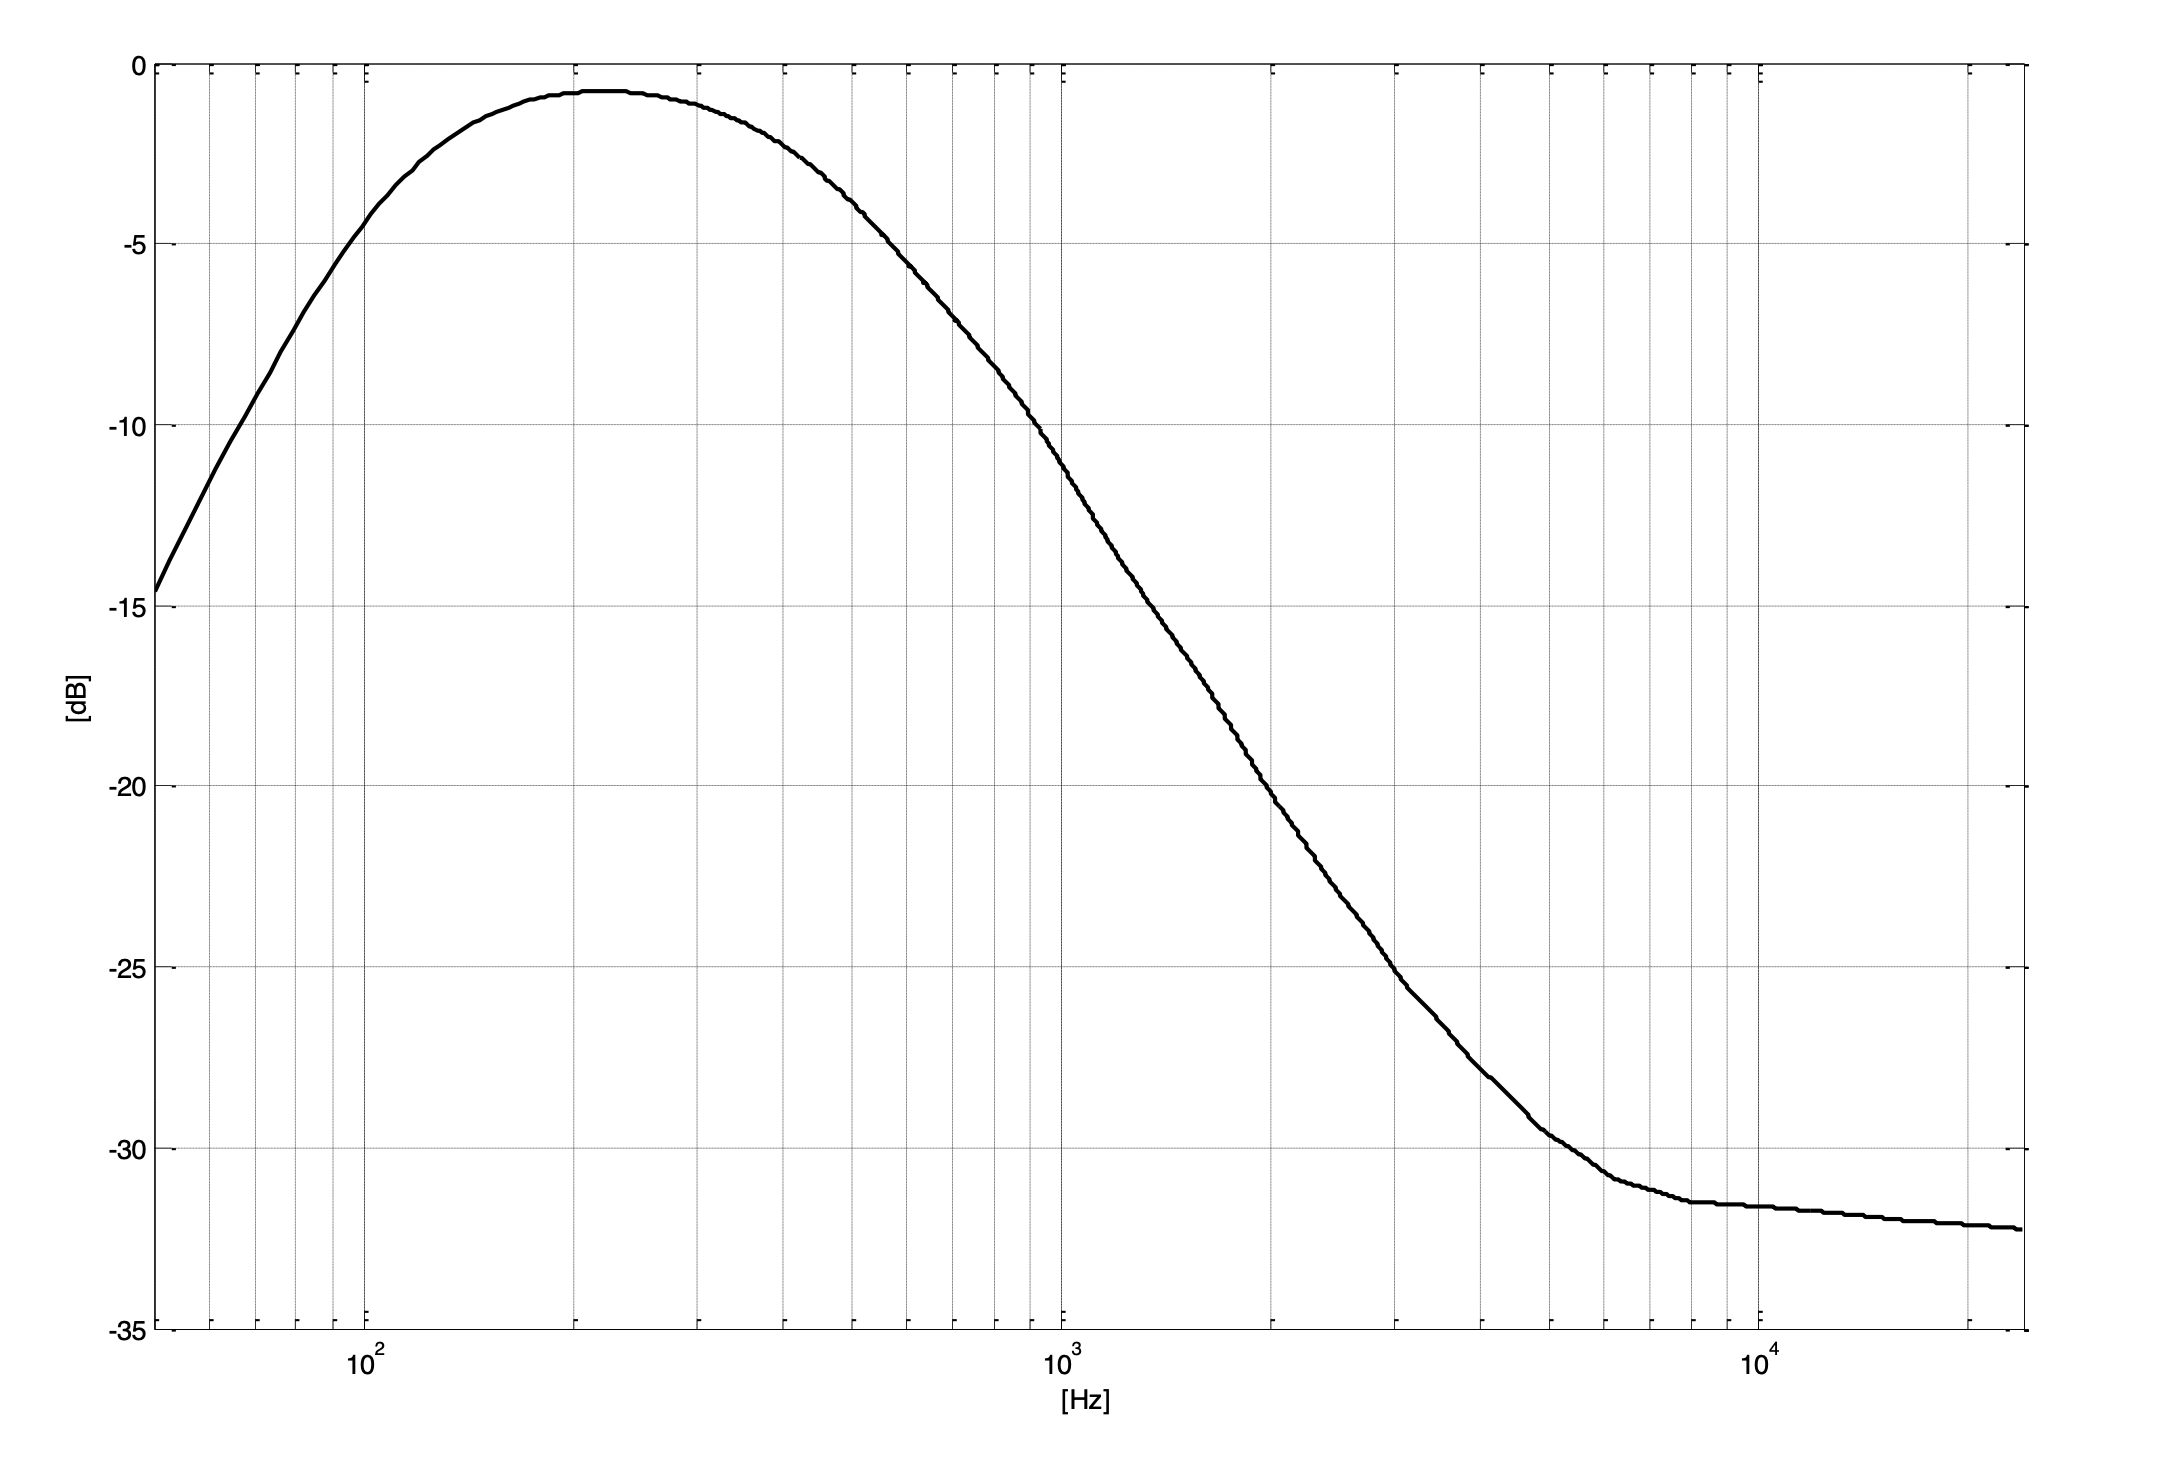
\includegraphics[width=\textwidth]{mnru-p50NoiseShape}
    \end{center}
    \caption{Frequency response of noise shaping filter.\label{MNRUP50}}
\end{figure}

Note that due to the noise shaping, an increase of the noise gain by +9dB is necessary in order to preserve the SNR as
defined by the Q parameter.
The noise shaping may be implemented using two cascaded IIR and FIR filters, where the IIR filter acts as a highpass
filter with a cutoff frequency of 115Hz (Table \ref{p50IIR}), and the FIR is used as a lowpass and band-shaping filter
(Table \ref{p50FIR}).

\begin{table}
    \centering
    \begin{tabular}{lrrr}
        a0..2 & 0.98941 & -1.97882 & 0.98941 \\
        b0..2 & 1.0 & -1.97871 & 0.97894 \\

    \end{tabular}
    \caption{IIR filter coefficients for noise shaping}
    \label{p50IIR}
\end{table}


\begin{table}
    \centering
    \resizebox{\textwidth}{!}{\begin{tabular}{lrlllllll}
        b\textsubscript{0..7} & 5.6159e-6 & 4.6163e-6 & 3.6904e-6 & 2.8871e-6 & 2.2044e-6 & 1.6539e-6 & 1.2084e-6 & 8.3224e-7 \\
        b\textsubscript{8..15} & 4.6748e-7 & 5.7472e-8 & -5.0130e-7 & -1.2669e-6 & -2.3140e-6 & -3.7063e-6 & -5.5290e-6 & -7.8631e-6 \\
        b\textsubscript{16..23} & -1.0843e-5 & -1.4513e-5 & -1.8887e-5 & -2.3912e-5 & -2.9539e-5 & -3.5739e-5 & -4.2634e-5 & -5.0323e-5 \\
        b\textsubscript{24..31} & -5.8925e-5 & -6.8454e-5 & -7.8831e-5 & -8.9844e-5 & -1.0135e-4 & -1.1310e-4 & -1.2493e-4 & -1.3673e-4 \\
        b\textsubscript{32..39} & -1.4845e-4 & -1.6008e-4 & -1.7183e-4 & -1.8377e-4 & -1.9603e-4 & -2.0867e-4 & -2.2175e-4 & -2.3527e-4 \\
        b\textsubscript{40..47} & -2.4940e-4 & -2.6406e-4 & -2.7915e-4 & -2.9440e-4 & -3.0961e-4 & -3.2452e-4 & -3.3921e-4 & -3.5341e-4 \\
        b\textsubscript{48..55} & -3.6669e-4 & -3.7825e-4 & -3.8720e-4 & -3.9268e-4 & -3.9462e-4 & -3.9308e-4 & -3.8856e-4 & -3.8146e-4 \\
        b\textsubscript{56..63} & -3.7217e-4 & -3.6064e-4 & -3.4739e-4 & -3.3241e-4 & -3.1609e-4 & -2.9860e-4 & -2.8033e-4 & -2.6118e-4 \\
        b\textsubscript{64..71} & -2.4157e-4 & -2.2077e-4 & -1.9795e-4 & -1.7182e-4 & -1.4162e-4 & -1.0692e-4 & -6.9224e-5 & -2.9565e-5 \\
        b\textsubscript{72..79} & 1.0779e-5 & 5.1586e-5 & 9.2954e-5 & 1.3597e-4 & 1.8033e-4 & 2.2716e-4 & 2.7767e-4 & 3.3456e-4 \\
        b\textsubscript{80..87} & 4.0054e-4 & 4.7887e-4 & 5.6936e-4 & 6.7180e-4 & 7.8421e-4 & 9.0553e-4 & 1.0351e-3 & 1.1753e-3 \\
        b\textsubscript{88..95} & 1.3266e-3 & 1.4923e-3 & 1.6746e-3 & 1.8757e-3 & 2.0950e-3 & 2.3324e-3 & 2.5833e-3 & 2.8472e-3 \\
        b\textsubscript{96..103} & 3.1256e-3 & 3.4247e-3 & 3.7501e-3 & 4.1090e-3 & 4.4978e-3 & 4.9144e-3 & 5.3546e-3 & 5.8206e-3 \\
        b\textsubscript{104..111} & 6.3167e-3 & 6.8548e-3 & 7.4344e-3 & 8.0591e-3 & 8.7259e-3 & 9.4382e-3 & 1.0199e-2 & 1.1025e-2 \\
        b\textsubscript{112..119} & 1.1914e-2 & 1.2873e-2 & 1.3901e-2 & 1.5002e-2 & 1.6175e-2 & 1.7446e-2 & 1.8795e-2 & 2.0241e-2 \\
        b\textsubscript{120..127} & 2.1785e-2 & 2.3466e-2 & 2.5289e-2 & 2.7347e-2 & 2.9502e-2 & 3.1675e-2 & 3.3583e-2 & 3.5567e-2 \\
        b\textsubscript{128..135} & 6.1233e-2 & 3.5567e-2 & 3.3583e-2 & 3.1675e-2 & 2.9502e-2 & 2.7347e-2 & 2.5289e-2 & 2.3466e-2 \\
        b\textsubscript{136..143} & 2.1785e-2 & 2.0241e-2 & 1.8795e-2 & 1.7446e-2 & 1.6175e-2 & 1.5002e-2 & 1.3901e-2 & 1.2873e-2 \\
        b\textsubscript{144..151} & 1.1914e-2 & 1.1025e-2 & 1.0199e-2 & 9.4382e-3 & 8.7259e-3 & 8.0591e-3 & 7.4344e-3 & 6.8548e-3 \\
        b\textsubscript{152..159} & 6.3167e-3 & 5.8206e-3 & 5.3546e-3 & 4.9144e-3 & 4.4978e-3 & 4.1090e-3 & 3.7501e-3 & 3.4247e-3 \\
        b\textsubscript{160..167} & 3.1256e-3 & 2.8472e-3 & 2.5833e-3 & 2.3324e-3 & 2.0950e-3 & 1.8757e-3 & 1.6746e-3 & 1.4923e-3 \\
        b\textsubscript{168..175} & 1.3266e-3 & 1.1753e-3 & 1.0351e-3 & 9.0553e-4 & 7.8421e-4 & 6.7180e-4 & 5.6936e-4 & 4.7887e-4 \\
        b\textsubscript{176..183} & 4.0054e-4 & 3.3456e-4 & 2.7767e-4 & 2.2716e-4 & 1.8033e-4 & 1.3597e-4 & 9.2954e-5 & 5.1586e-5 \\
        b\textsubscript{184..191} & 1.0779e-5 & -2.9565e-5 & -6.9224e-5 & -1.0692e-4 & -1.4162e-4 & -1.7182e-4 & -1.9795e-4 & -2.2077e-4 \\
        b\textsubscript{192..199} & -2.4157e-4 & -2.6118e-4 & -2.8033e-4 & -2.9860e-4 & -3.1609e-4 & -3.3241e-4 & -3.4739e-4 & -3.6064e-4 \\
        b\textsubscript{200..207} & -3.7217e-4 & -3.8146e-4 & -3.8856e-4 & -3.9308e-4 & -3.9462e-4 & -3.9268e-4 & -3.8720e-4 & -3.7825e-4 \\
        b\textsubscript{208..215} & -3.6669e-4 & -3.5341e-4 & -3.3921e-4 & -3.2452e-4 & -3.0961e-4 & -2.9440e-4 & -2.7915e-4 & -2.6406e-4 \\
        b\textsubscript{216..223} & -2.4940e-4 & -2.3527e-4 & -2.2175e-4 & -2.0867e-4 & -1.9603e-4 & -1.8377e-4 & -1.7183e-4 & -1.6008e-4 \\
        b\textsubscript{224..231} & -1.4845e-4 & -1.3673e-4 & -1.2493e-4 & -1.1310e-4 & -1.0135e-4 & -8.9844e-5 & -7.8831e-5 & -6.8454e-5 \\
        b\textsubscript{232..239} & -5.8925e-5 & -5.0323e-5 & -4.2634e-5 & -3.5739e-5 & -2.9539e-5 & -2.3912e-5 & -1.8887e-5 & -1.4513e-5 \\
        b\textsubscript{240..247} & -1.0843e-5 & -7.8631e-6 & -5.5290e-6 & -3.7063e-6 & -2.3140e-6 & -1.2669e-6 & -5.0130e-7 & 5.7472e-8 \\
        b\textsubscript{248..255} & 4.6748e-7 & 8.3224e-7 & 1.2084e-6 & 1.6539e-6 & 2.2044e-6 & 2.8871e-6 & 3.6904e-6 & 4.6163e-6 \\
        b\textsubscript{256} & 5.6159e-6 &  &  &  &  &  &  &  \\
    \end{tabular}}
    \caption{FIR filter coefficients for noise shaping}
    \label{p50FIR}
\end{table}

\subsection {Implementation}

The implementation of fullband noise-shaped MNRU is provided in {\tt mnru} directory.
{\tt P50\_MNRU\_process() } in {\tt mnru.c} provides the main algorithm,
{\tt filter\_coeffs.c} provides the IIR and FIR filter routines,
and {\tt filter\_coeffs.h} gives the filter coefficients as described in Tables \ref{p50IIR} and \ref{p50FIR}.

{\tt p50fbmnru.c} provides code for the command line tool, similar to {\tt mnrudemo.c} for NB and WB MNRU.

The usage for the command line tool is as follows:

{\tt p50fbmnru <inputfile> <outputfile> <Q/dB> <Mode> [dcFilterOn]}

{\tt inputfile} is the path to the PCM 16-bit 48kHz input signal.

{\tt outputfile} is the path to the PCM 16-bit 48kHz output signal.

{\tt Q/dB} is the target SNR level {\tt Q}.

{\tt Mode} defines the output signal:
\begin{itemize}
    \item {\tt M} outputs the input signal with added modulated noise.
    \item {\tt N} outputs the modulated noise only.
    \item {\tt S} outputs a copy of the input signal.
\end{itemize}

{\tt [dcFilterOn]} is an optional parameter
\begin{itemize}
    \item {\tt 0} disable DC Filter (default and recommended)
    \item {\tt 1} enable DC Filter
\end{itemize}


